% ------------------------------------------------------------------------
%	Latex Preamble:  Formatting and Custom Commands
% ------------------------------------------------------------------------
\documentclass[12pt]{article}

\usepackage{amsmath, graphicx, subfig}

% to control the page number location and running title
\usepackage{fancyhdr}

% For the draft
\usepackage{endfloat}

% To control the spacing
\usepackage{setspace}

% For including code1
\usepackage{listings}

% For using URLs
\usepackage{url}

% Citations are numbers, with round parenthesis
% no brackets around numbers in the bibliography
% use the CBE/CSE bib style
\usepackage[numbers,round]{natbib}
\renewcommand{\bibnumfmt}[1]{#1.}
\bibliographystyle{mrm}

% Equations have square brackets around them
\makeatletter
  \def\tagform@#1{\maketag@@@{[#1]\@@italiccorr}}
\makeatother

% Spacing and indentation
\topmargin -0.4in
\headheight 0.45in
\oddsidemargin 0in
\evensidemargin 0in
\textwidth 6.5in
\textheight 9in

\setlength{\parindent}{0pt} % No paragraph indent.
\setlength{\parsep}{12pt}   % Paragraph separation.
\setlength{\parskip}{12pt}  % Paragraph skip.

% Set the graphics path
\graphicspath{{./figures/}}


% ------------------------------------------------------------------------
%	Document start
% ------------------------------------------------------------------------
\begin{document}

\lhead{ISMRM Raw Data Format}
\chead{}
\rhead{\thepage}
\lfoot{}
\cfoot{}
\rfoot{}

% ------------------------------------------------------------------------
%	Full Title Page
% ------------------------------------------------------------------------
\newpage
\clearpage
\pagestyle{empty}
\vspace*{20mm}

\begin{center}
\large \textbf{ISMRM Raw Data Format: A Proposed Standard for Sharing MRI Raw Datasets}

\normalsize
\singlespacing
Souheil J. Inati$^1$,
Joseph D. Naegele$^1$, 
Nicholas R. Zwart$^2$,
Vinai Roopchansingh$^1$,
Martin J. Lizak$^3$,
David Hansen$^3$,
David Atkinson$^4$,
Peter Kellman$^5$,
Sebastian Kozerke$^6$,
Hui Xue$^5$,
Thomas S. Sorensen$^3$,
James G. Pipe$^2$,
Michael S. Hansen$^5xs$
\end{center}

\begin{enumerate}
\item National Institute of Mental Health, National Institutes of Health, Bethesda, MD
\item Keller Center for Imaging Innovation, Barrow Neurological Institute, Phoenix, AZ
\item National Institute of Neurologic Disease and Stroke, National Institutes of Health, Bethesda, MD
\item Department of Computer Science, Aarhus University, Aarhus, Denmark
\item Centre for Medical Image Computing, University College London, United Kingdom
\item National Heart, Lung, and Blood Institute, National Institutes of Health, Bethesda, MD
\item Institute for Biomedical Engineering, University and ETH Zurich, Zurich, Switzerland
%\item Institute of Neuroscience and Medicine, Medical Imaging Physics, Forschungszentrum Julich, Ju�lich, Germany
%\item Philips Research Laboratories, Hamburg, Germany
%\item Department of Biomedical Engineering and Department of Medical Physics, University of Wisconsin, Madison, Wisconsin
%\item Department of Radiology, University Hospitals of Cleveland, Cleveland, OH
%\item Department of Radiological Sciences, University of California Los Angeles, Los Angeles, California, USA
%\item Department of Biomedical Engineering, University of Virginia, Charlottesville, VA
%\item Department of Biomedical Engineering, University of Michigan, Ann Arbor, MI
\end{enumerate}

\vspace{5mm}
Correspondence to: \\
Souheil J. Inati \\
National Institue of Mental Health, NIH \\
NIH Building 10/1D-70 \\
10 Center Drive \\
Bethesda, MD 20892 \\
\textit{souheil.inati@nih.gov} \\

\textit{Running Head:  ISMRMRD}

\vspace{5mm}

\textit{Submitted to Magnetic Resonance in Medicine} 

% ------------------------------------------------------------------------
%	Abbreviated Title Page
% ------------------------------------------------------------------------
\newpage
\clearpage
\pagenumbering{arabic} % begin numbering here
\pagestyle{fancy}
\begin{center}
\vspace*{70mm}
\large \textbf{ISMRM Raw Data Format: A Proposed Standard for Sharing MRI Raw Datasets} \\
\end{center}
\normalsize 

\textit{Running Head:  ISMRMRD}

\vspace{5mm}

\textit{Submitted to Magnetic Resonance in Medicine} 

\textit{Word count:  }  

% ------------------------------------------------------------------------
%	Abstract
% ------------------------------------------------------------------------
\newpage
\clearpage
\doublespacing
\section*{Abstract}
\textbf{Purpose:}
A common raw data format is a prerequisite for sharing MR image reconstruction algorithms and code, and is a necessary component of reproducible research.  Ideally, this common format would be vendor neutral, and would capture the data fields needed to describe the details of the MR experiment so as to permit image reconstruction from the raw data.  We propose the ISMRM Raw Data (ISMRMRD) format as an example of such a common raw data format.\\
\textbf{Methods:}  The proposed \\
\textbf{Results:} Data demonstrate \\
\textbf{Conclusion:} The proposed raw data format solves a practical problem.

\textit{Abstract word count: }  

% ------------------------------------------------------------------------
%	Keywords
% ------------------------------------------------------------------------
\textbf{Keywords:}  Image reconstruction, Open Source, Raw Data Format

% ------------------------------------------------------------------------
%	Body
% ------------------------------------------------------------------------
\newpage
\clearpage
\onecolumn

% ------------------------------------------------------------------------
%	Introduction
% ------------------------------------------------------------------------
\section*{Introduction}
Image reconstruction research has played a pivotal role in driving many advances in magnetic resonance imaging. Examples of paradigm shifting techniques include parallel imaging~\cite{Pruessmann:1999uq, Sodickson:1997fk, Griswold:2002kx}  and more recently the introduction of compressed sensing~\cite{Donoho:2006compressed, Lustig:2007vn}. Novel reconstruction algorithms build on and improve existing methodology and most reconstruction articles compare new methods to existing methods in terms of image quality and reconstruction speed.

Reproducible research has drawn a great deal of attention recently, as highlighted for example in a recent special issue of Science~\cite{Jasny:2011again, Peng:2011reproducible}. The field of computational science in particular has produced several excellent examples of how such research can be carried out, e.g. the wavelab toolbox~\cite{wavelab}.  The ISMRM has begun to take steps to help to facilitate reproducible research, e.g. with the MRI unbound website~\cite{mri_unbound}. Underlying many of these efforts is a discipline specific file format specification that allows scientists to easily exchange data.  Much of modern astronomy research, for example, relies on telescope data in the FITS standard~\cite{fits}.  Other discipline specific data formats have enabled scientists to escape from the limitations imposed by vendor specific proprietary technology, leading to the development of a wide range of post acquisition data analysis tools, and enabling large scale collaborations.  Medical imaging has the DICOM standard~\cite{dicom}, which allows radiology departments to store data from different vendors on a centralized PACS, and computer scientists to implement novel image processing methods in a vendor neutral manner. The subfield of neuroimaging has NIfTI~\cite{nifti}, which underlies large scale projects like the human connectome project~\cite{connectome}.  For the field of MRI, these image file formats serve well, but they do not address the needs of practitioners involved in the development of image reconstruction algorithms, nor do they store the data in a format that is very closely tied to the instrument and to the particulars of the MR experiment. We believe that a first and necessary step is the development of a MR specific raw data file format.

This ISMRMRD standard was developed by a subcommittee of the ISMRM Sedona 2013 workshop.  It is designed to capture the details of the MRI experiment in a way that permits image reconstruction.  It is important to note that this goal is fundamentally different from that of proprietary vendor raw data file formats.  Generally speaking, proprietary vendor raw file formats are intended to capture protocol parameters and the state of the scanner graphical user interface (GUI) for a particular pulse sequence at the time of the scan.  The proprietary vendor raw data file formats are intended to store the information needed to reproduce a particular experiment on a specific version of the scanner software version, and to enable image reconstruction within that same scanner's image reconstruction software framework.  Because of the tight coupling between 1) the scanner console user interface, 2) the pulse sequence and the pulse sequence control parameters, and 3) the image reconstruction software and the image reconstruction software control parameters, the  vendor raw data file formats depend on and contain a great deal of proprietary vendor specific knowledge making the unsuitable for data sharing.  More importantly, the specific implementation details of a particular vendors' scanner software architecture greatly influences the design of these file formats and the type of information that they contain.  The ISMRMRD standard on the other hand is designed to permit the exchange of the raw k-space data and a description of the physics of the data acquisition process, at least in so far as image reconstruction is concerned.  NEED MORE HERE.


% ------------------------------------------------------------------------
%	Methods
% ------------------------------------------------------------------------
\section*{Architecture and Implementation}
\subsection*{Design}
The ISMRMRD format combines a mix of flexible data structures (XML header) and fixed structures (equivalent to C-structs).  A minimal raw data set consists of two sections:
\begin{itemize}
\item{XML header} A flexible XML format document that can contain an arbitrary number of fields and accommodate everything from simple values (b-values, etc.) to entire vendor protocols, etc. This purpose of this XML document is to provide parameters that may be meaningful for some experiments but not for others. This XML format is defined by an XML Schema Definition file (ismrmrd.xsd).
\item{Raw data} This section contains all the acquired data in the experiment organized as a sequence of data items.  Each data item corresponds to a single frame or chunk in an experiment, for example a single line of data in a cartesian acquisition or a single interleave in a multi-shot spiral acquisition. Each data item consists of a fixed size header (C-struct) with encoding numbers, etc., along with the k-space data for all of the each acquired channel, and (optionally) the k-space trajectory. The raw data headers are defined in a C/C++ header file (ismrmrd.h)
\end{itemize}

The format supports storing k-space trajectories along with the data and provides a simple image format for storing the product of reconstructions.

We should describe in more detail:
\begin{itemize}
\item Encoding spaces
\end{itemize}

\subsection*{ISMRMRD Library}
We have created an implementation of this standard using HDF5 files for storage, along with C, C++, Python and MATLAB, libraries for reading and writing ISMRMRD files.  The project follows an open source development model with a website at http://ismrmrd.github.io and a discussion board and code repositories at http://github.com/ismrmrd.  

As shown schematically below, the HDF5 container stores the variable length (extensible) XML header, followed by header/data pairs, where each fixed length header (c-struct) encodes readout specific information (k-space location, slice, etc).

The XML header can be thought of as a text representation of a data structure and there are many ways to:
\begin{itemize}
\item generate the text representation from the data structure (serialization), and
\item parse the text representation and populate the fields of the data structure (deserialization)
\end{itemize} 
One could chose to generate an XML header by hand (e.g. with a text editor), although this is useful for prototyping it is generally inconvenient for production.  There are two different strategies for creating the data structure corresponding to the XML structure described by the schema file and the serialization and deserialization functions needed to go between the text and the data structure.  One could either hand craft code, or use XML data binding and process the schema file to auto-generate source code for an object that can be serialized into an XML string or deserialized from an XML string.   The tradeoff between hand crafted and auto-generated code depends a great deal on the available tools.  Generally speaking hand crafting code allows for the creation of a better API for the end user, at the expense of (potentially) a great deal of effort on the part of the library authors, whereas auto-generating code is significantly less effort on the part of the library authors and guarantees the generation of valid XML strings that conform to the schema, but results in often awkward and inconvenient syntax for the end user .  We explored various options for each language: Code Synthesis XSD  for C++, JAXB for JAVA as MATLAB can use JAVA objects directly, and PyXB for Python.  As of this writing, we have chosen to hand craft the code for C++ and JAVA and to auto-generate the code for Python.

\subsubsection{C implementation}
Depends on HDF5.

\subsubsection{C++ implementation}
Wrapper around the C library and hand crafted XML header binding class.

\subsubsection{Python implementation}
The PyXB generated XML header binding class.  H5Py for interacting with the files.  Numpy arrays for the data and the k-space trajectories.

\subsubsection{Matlab implementation}
Hand crafted JAVA code for the XML header binding class.
Matlab ships with a version of the HDF5 library.
An implementation using pure matlab functions (with the Mathworks provided HDF5 interface).


% Figure 1
\begin{figure}
\label{fig:format}
\begin{center}
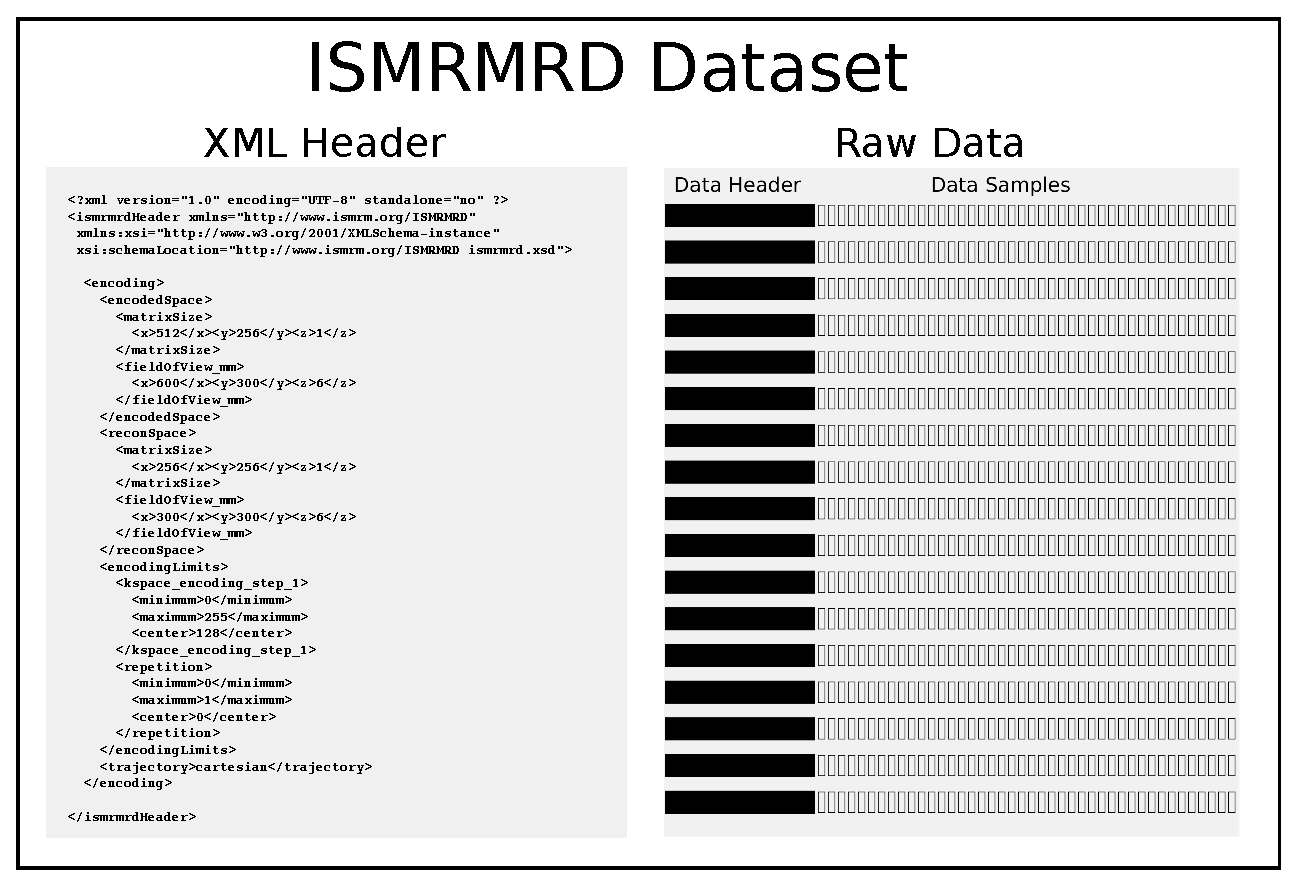
\includegraphics[width=6in]{ismrmrd_format.eps}
\caption{HDF5 File Format}
\end{center}
\end{figure}

% Figure 2
\begin{figure}
\label{fig:encoding}
\begin{center}
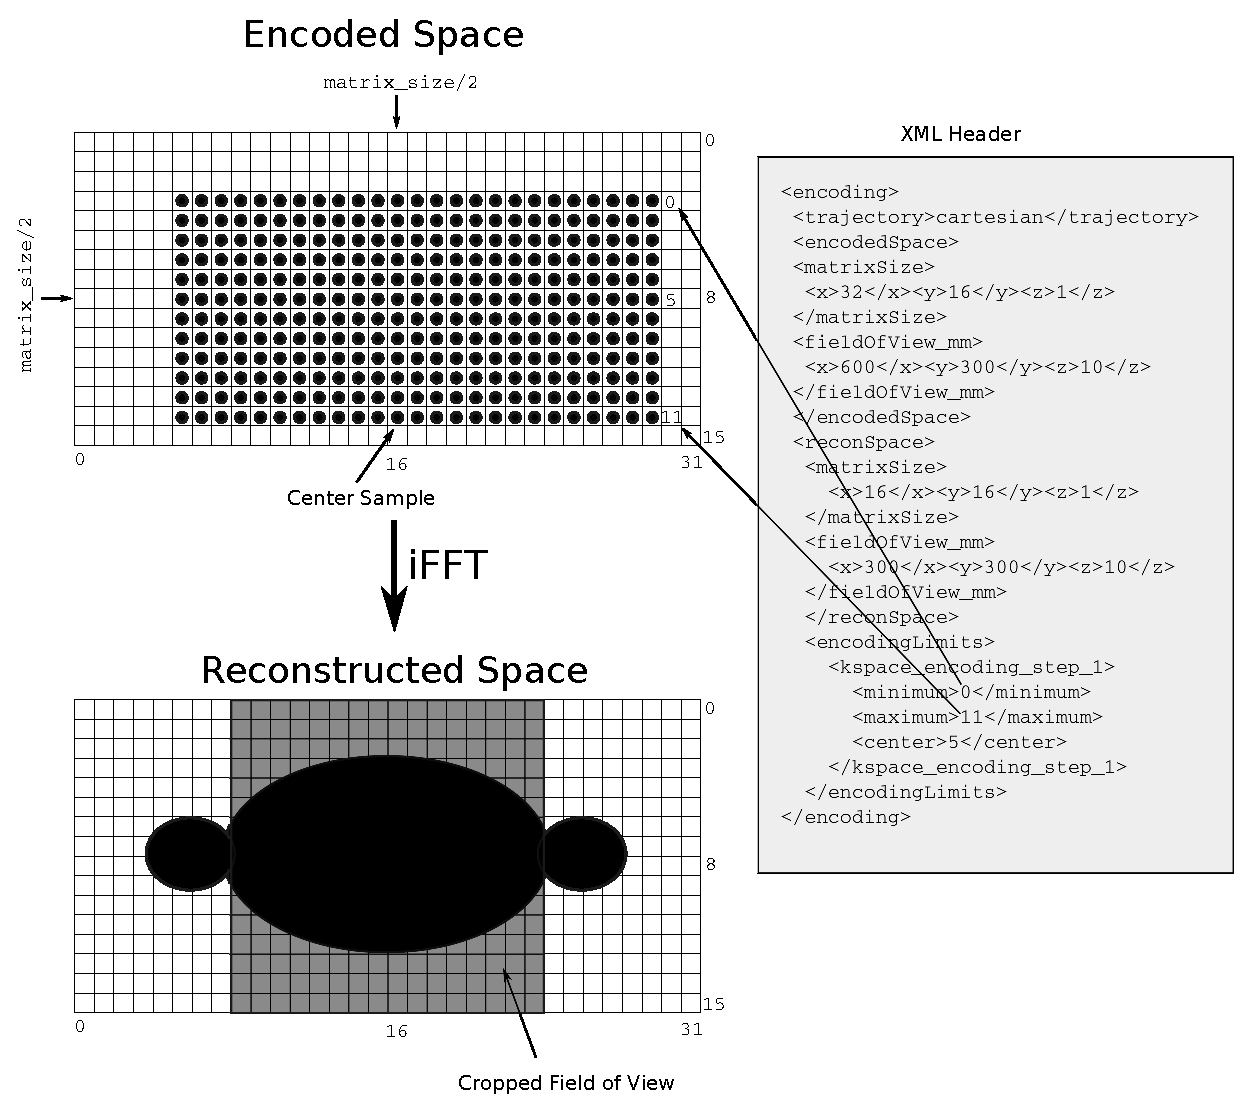
\includegraphics[width=6in]{encoding_spaces.eps}
\caption{Encoding spaces:}
\end{center}
\end{figure}

% Figure 3
\begin{figure}
\label{fig:cstruct}
\begin{center}
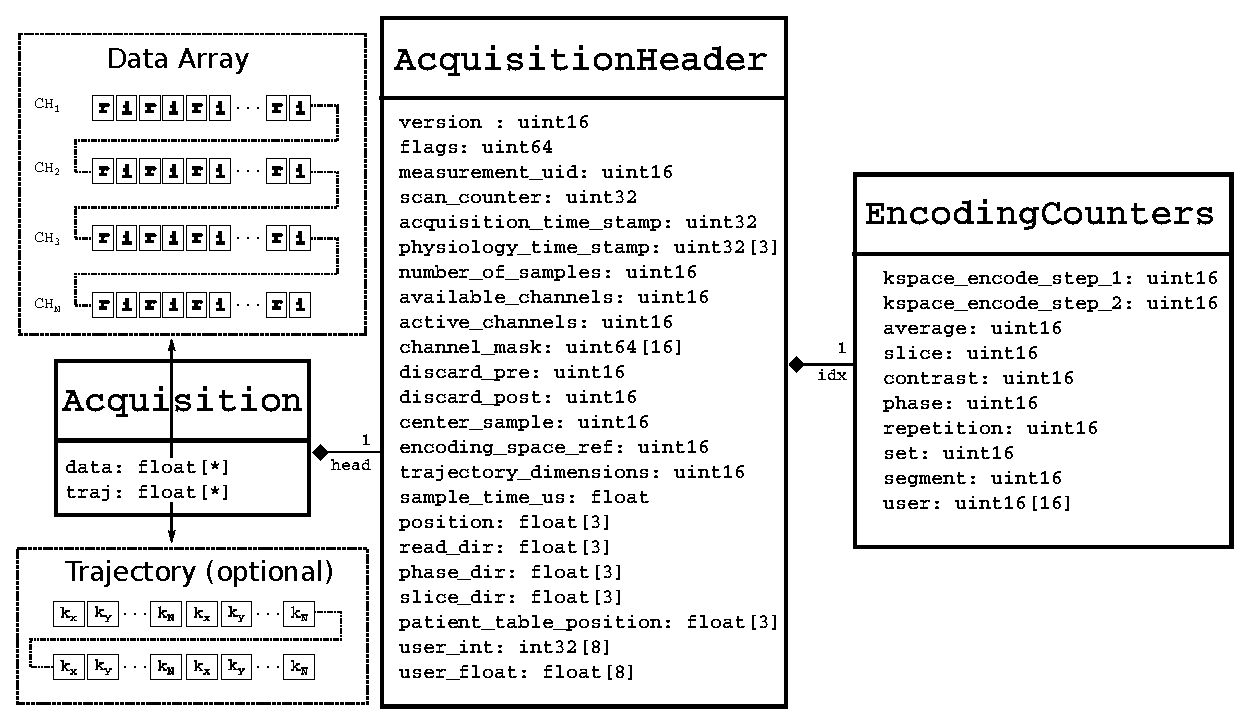
\includegraphics[width=6in]{uml_diagram.eps}
\caption{Data header structure}
\end{center}
\end{figure}

\subsection*{Vendor Specific Tools}
We have developed converters for several vendors proprietary file formats: Bruker, General Electric, Philips, and Siemens.  The Bruker, Philips and Siemens converters are open source with repositories that can also be found at http://github.com/ismrmrd.  The GE converter relies on proprietary vendor code and are being distributed via the vendor's research network.  Given the variety in vendor raw data file formats, we  describe the architecture of these programs in general terms in the hope of providing some guidance or aid to others who are implementing their own conversion tools.  We refer the reader to the source code for  details.  Roughly speaking, Bruker raw data is stored in a simple directory structure with the acquisition parameters stored in several text files and k-space data stored in a simple binary file as equal length frames of k-space data (without tags).  Siemens raw data files on the other hand have a more complicated structure.  A single file can store raw data from multiple scans.  For each scan, acquisition parameters are stored in a structured text header, followed by k-space data frames stored in acquisition order, where each frame of k-space data is tagged with a small header containing the frame's line number, slice number, location, etc.  Philips and GE raw data files are organized in structures of intermediate complexity.

The four converters were written in C++.  The acquisition parameters (structured text header or binary data structures) were converted to XML (containing vendor specific parameter names and parameter values).  This XML file was then processed with a sequence specific XSL style sheet to convert the vendor specific parameters into the vendor independent ISMRMRD XML header.  The frames of k-space data were processed in the order in which they appeared on disk.  For vendors with tagged data frames, the proprietary binary header tag was parsed and used to populate the ISMRMRD AcquisitionHeader structure.  For vendors with untagged data frames, sequence and vendor specific knowledge was used.  

It is worth emphasizing that these converters required some work and a good deal of vendor specific knowledge on the part of the developers.  However, once code was developed for converting raw data from one pulse sequence on a particular platform, it was quite straightforward to modify this code to handle other sequences and we believe that others can easily modify these converters to handle currently unsupported product sequences or their own research sequences.

\section*{Experimental Demonstration}

In a typical MR image reconstruction research project, one would like to test and/or validate an algorithm and an implementation on simulated data and on data acquired from a phantom or from an in-vivo experiment.  Here we demonstrate how one could use the ISMRMRD format and APIs in a prototypical image reconstruction research project: the development, implementation and testing of a trivial image reconstruction algorithm suitable for 2D experiments in which the k-space data are acquired on a fully sampled cartesian grid.  The workflow for this toy research project is depicted in fig.~\ref{fig::workflow}.  It is a subset of a more complete full development cycle:
\begin{enumerate}
\item An initial implementation or proof of concept of the algorithm is implemented in a rapid prototyping language such as Matlab or Python.
\item Synthetic data are generated in simulation and used to test/validate the prototype implementation.
\item Real (experimental) data are collected and used to test/validate the prototype implementation.
\item A high performance/production version of the algorithm is implemented in a compiled language such as C/C++ or Fortran.  In some cases the high performance implementation may require specialized hardware such a compute cluster or a graphical processing unit (GPU).
\item The synthetic and real data sets are used to test/validate the high performance implementation of the algorithm.
\item The high performance implementation of the algorithm is put into production in a clinical environment.
\end{enumerate}

In the interest of reproducible research, the authors of the publication describing the implementation and validation of this image reconstruction algorithm will distribute the source code for the implementation of the algorithm and the raw data sets that were used to generate the figures for the publication and perhaps additional code or data related to the testing or validation of the algorithm.

% Figure 4
\begin{figure}[ht]
\begin{center}
\includegraphics[width=6in]{recon_demo}
\end{center}
\caption{Experimental demonstration:  Data sets were acquired on scanners from four vendors and converted from the vendor proprietary raw data file formats into ISMRMRD format.  A fifth data set was synthesized numerically and stored in ISMRMD format.  The five ISMRMRD raw data sets were reconstructed using three image reconstruction programs written in C++, Matlab, and Python.  The resulting images are shown above, from left to right Bruker, General Electric, Philips, Siemens, and the synthetic data set,  and from top to bottom C++, Matlab, and Python reconstruction programs.}
\label{fig:demo}
\end{figure}

Our prototypical image research project begins with an outline of the steps of the toy algorithm:
\begin{enumerate}
\item data are read and stored in a buffer (Nkx,Nky,Nz)
\item the fourier transform is computed on the first two dimensions (x,y)
\item chop if the data were acquired on an oversampled grid in the frequency encode direction
\end{enumerate}
The prototype implementation of this algorithm was written in Python and Matlab.  The high performance implementation of the algorithm was written in C++.  All three implementations used the ISMRMRD API to read in an ISMRMRD format file.

Synthetic data sets were generated from a simple MR physics simulation of a GRE experiment collecting data from a single slice object (a Shepp-Logan phantom) using an 8-element birdcage coil.  Different instances of randomly generated white gaussian noise were added to the k-space data to simulate several repetitions of the experiment in the presence of noise.  The resulting simulated data sets were written to disk in ISMRMRD formats.  The simulation programs were implemented in C++, Python, and Matlab. 

Two real data sets were collected from a water phantom on two different 3T scanners: 1) a Siemens Skyra, and 2) a GE MR750.  Data were acquired using each vendor's product 2D gradient echo pulse sequence and 32 channel head coil.  The acquisition parameters were matched as closely as possible FOV=256~mm, slice thickness=5~mm, Nx=128, Ny=128, Nz=30, TR=250~ms, TE=min.  The raw data files were transferred off-line and converted into ISMRMRD using the vendor specific converters described above.

The ISMRMRD source code distribution (Sourceforge URL, hash) contains code for the image reconstruction programs and the raw data simulation programs.  It also contains the LaTeX source for this manuscript.  The source code for the raw data converters is being distributed through each vendor's research collaboration network.  The converted raw data in the vendor neutral ISMRMD format are being distributed via XNAT (URL).  

% ------------------------------------------------------------------------
%	Discussion
% ------------------------------------------------------------------------
\section*{Discussion and Conclusion}
We have presented an initial attempt at creating a standard for storing raw MR data and have demonstrated an implementation that supports several common programming languages.  We believe that as this standard is refined and evolves it will serve as a foundation upon which practitioners can base reproducible research project and collaborations.  A great deal of work remains and we ask for input from the ISMRM community to help shape the direction of the format.

% ------------------------------------------------------------------------
%	Acknowledgments
% ------------------------------------------------------------------------
\section*{Acknowledgements}
Multiple people participated in the discussions that led to this work.  We would like to acknowledge their contribution (in no particular order) 
Walter F. Block,
Peter Boernert,
David O. Brunner,
Mark A. Griswold,
Brian A. Hargreaves,
Craig H. Meyer,
Sonia Nielles-Vallespin,
Tim Nielsen and 
Douglas C. Noll.


% ------------------------------------------------------------------------
%	References	
% ------------------------------------------------------------------------
\bibliography{ismrmrd}

\end{document}
